
\begin{frame}
    \frametitle{Task-Specific Protein Language Models}
    \begin{columns}
        % Left Column: Tasks
        \column{0.45\textwidth}

        \begin{center}
            \begin{tikzpicture}[
                node distance=0.3cm and 1.2cm,
                align=center,
                rounded corners,
                every node/.style={},
                input/.style={draw, fill=lightblue2!50, text width=4cm, minimum height=1.5cm},
                arrow/.style={-Stealth, thick},
                scale=0.8
            ]

            % Tasks
            \visible<1>{\node[input, opacity=1] (structure) {Structure Determination};}
            \visible<2->{\node[input, opacity=.2] (structure) {Structure\\ Determination};}
            
            \visible<2>{\node[input, below=0.5cm of structure, opacity=1] (interactions) {Protein-Protein\\Interactions};}
            \visible<1, 3->{\node[input, below=0.5cm of structure, opacity=.2] (interactions) {Protein-Protein\\Interactions};}
            
            \visible<3>{\node[input, below=0.5cm of interactions, opacity=1] (mutation) {Mutation Effect\\ Prediction};}
            \visible<1-2,4->{\node[input, below=0.5cm of interactions, opacity=.2] (mutation) {Mutation Effect\\ Prediction};}
            
            \visible<1-3>{\node[input, below=0.5cm of mutation, opacity=.2] (design) {De novo\\ Protein Design};}
            \visible<4>{\node[input, below=0.5cm of mutation, opacity=1] (design) {De novo\\ Protein Design};}

        \end{tikzpicture}
        \end{center}

        % Right Column: Models
        \column{0.55\textwidth}
        \begin{center}
            \begin{tikzpicture}[
                node distance=0.3cm and 1,
                align=center,
                rounded corners,
                every node/.style={},
                input/.style={draw, fill=greyblue!40, text width=4cm, minimum height=.8cm},
                output/.style={draw,fill=white!10, text width=5cm, minimum height=.8cm},
                arrow/.style={-Stealth, thick},
                scale=0.8
            ]
            \only<1>{
                % \node {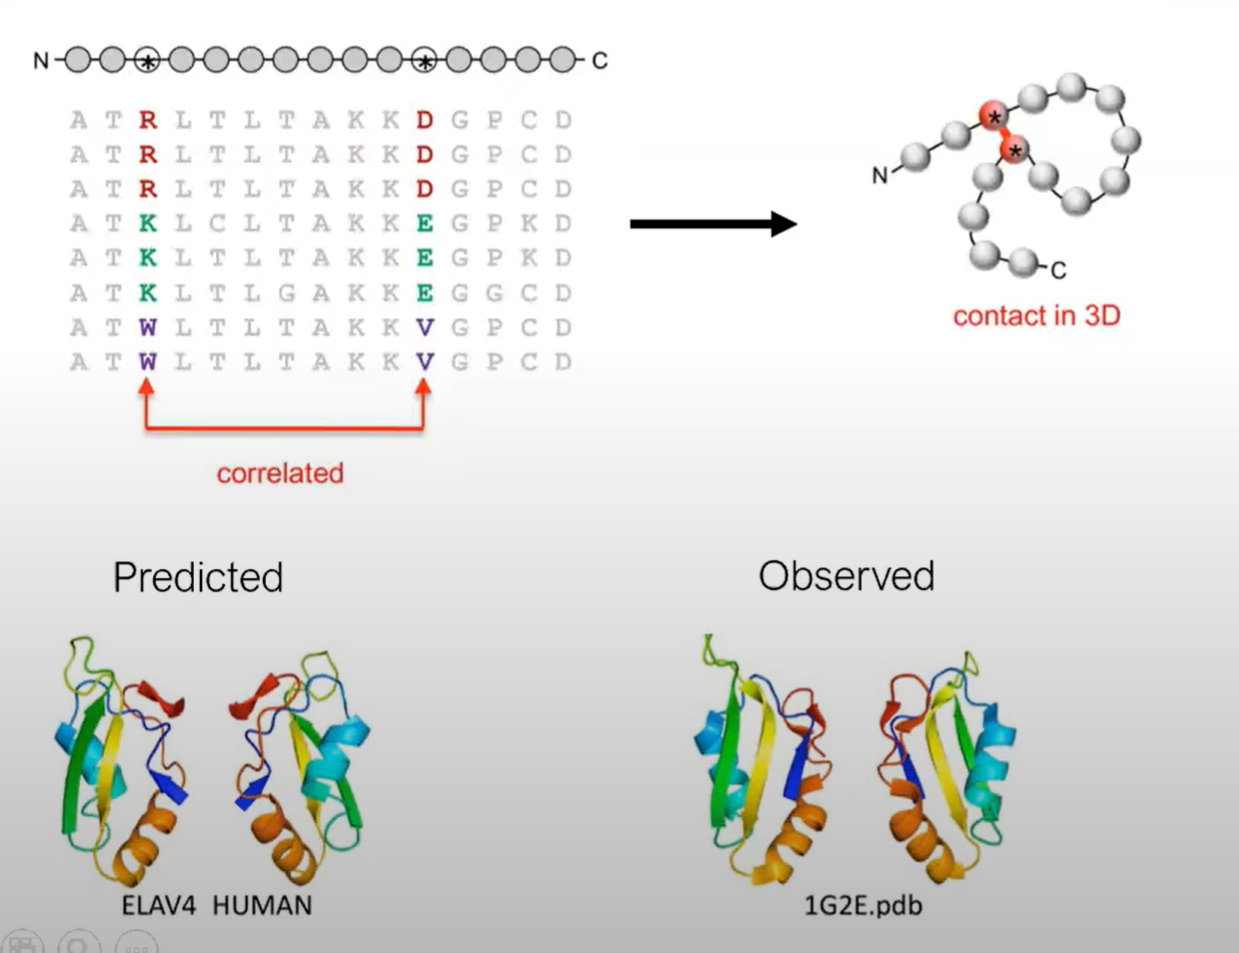
\includegraphics[width=\textwidth]{images/stdetr.png}};
                \node[input,text=black](alph) at (0,3.5)
                {AlphaFold};
                \node[below=.25cm of alph](alpic) {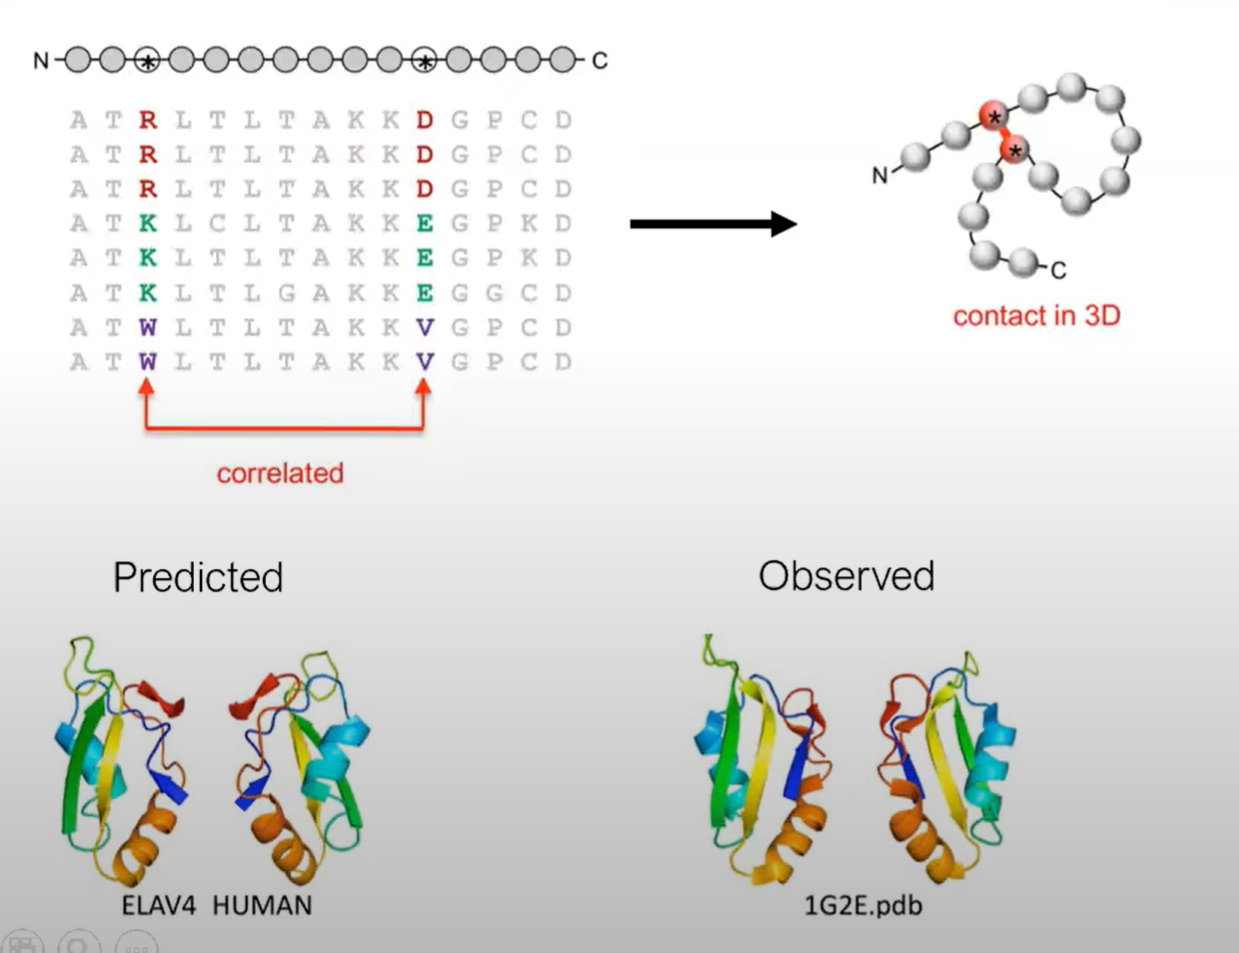
\includegraphics[width=5cm, keepaspectratio]{images/stdetr.png}};
                 \node[below=.25cm of alpic] at (alpic.south)
                {Aids in drug discovery, understanding\\ disease mechanisms and designing\\ therapeutic proteins};
            }
             \only<2>{
                \node[input,text=black](ppi) at (0,3.5)
                {DeepPPI};
                \node[below=.25cm of ppi](pipic) {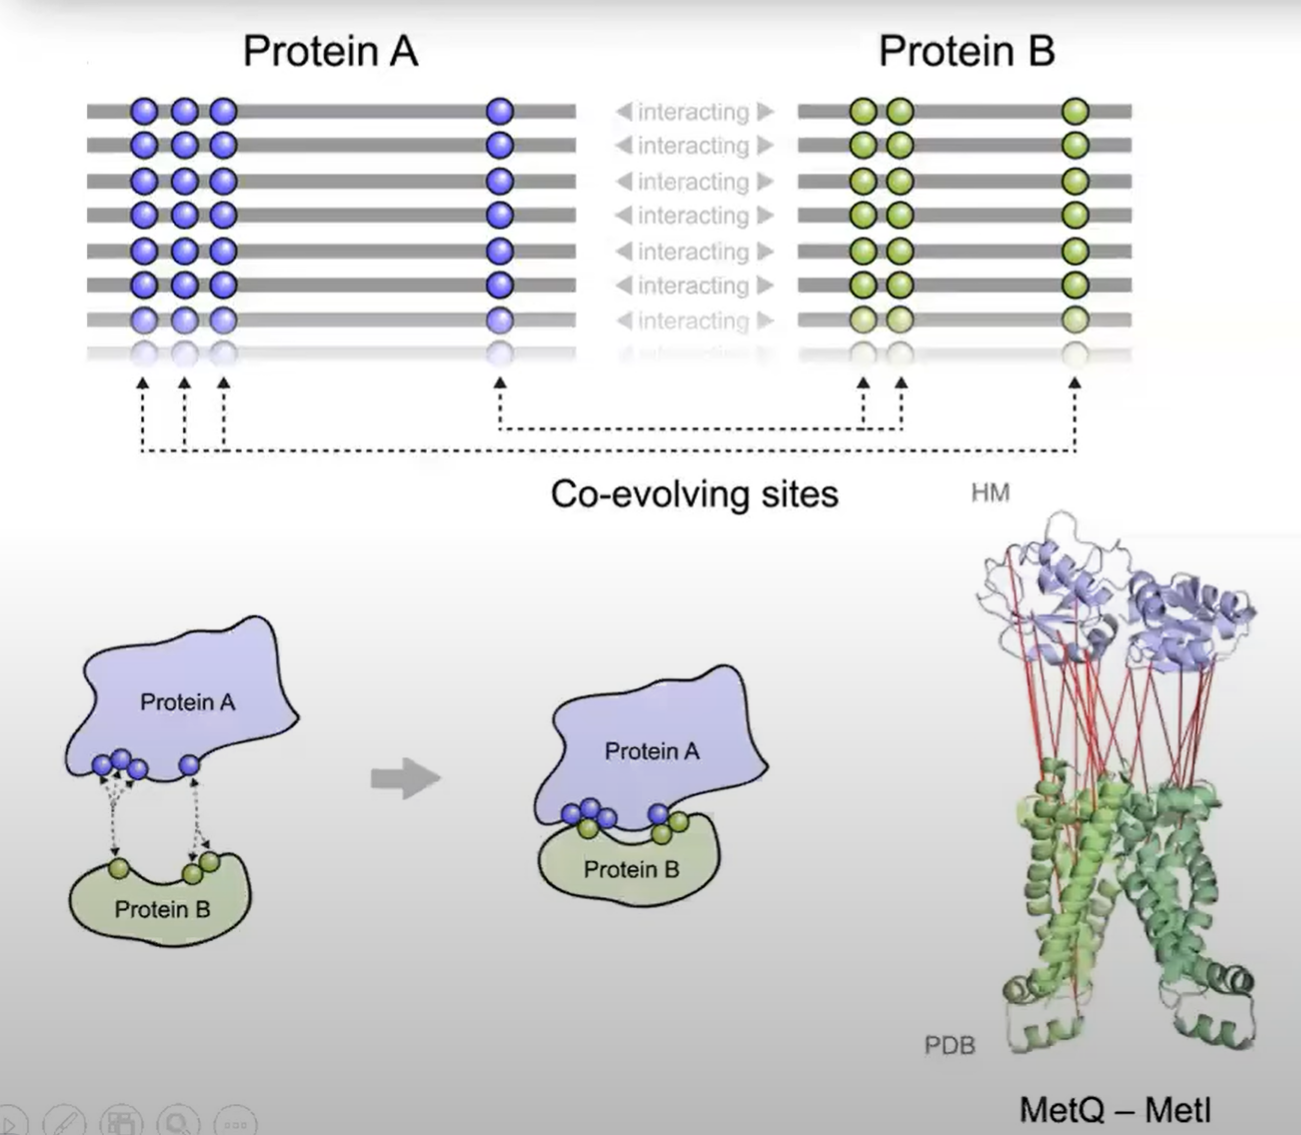
\includegraphics[width=5cm, keepaspectratio]{images/ppi.png}};
                 \node[below=.25cm of pipic] at (pipic.south)
                {Predicts how pathogen proteins\\ interact with human proteins,\\ guiding antiviral/antibacterial \\drug development};
            }
            \only<3>{
                \node[input,text=black](eve) at (0,3.5)
                {EVE \\(Evolutionary Model of Variant Effect Prediction)};
               \node[below=.25cm of eve] (mutpic) {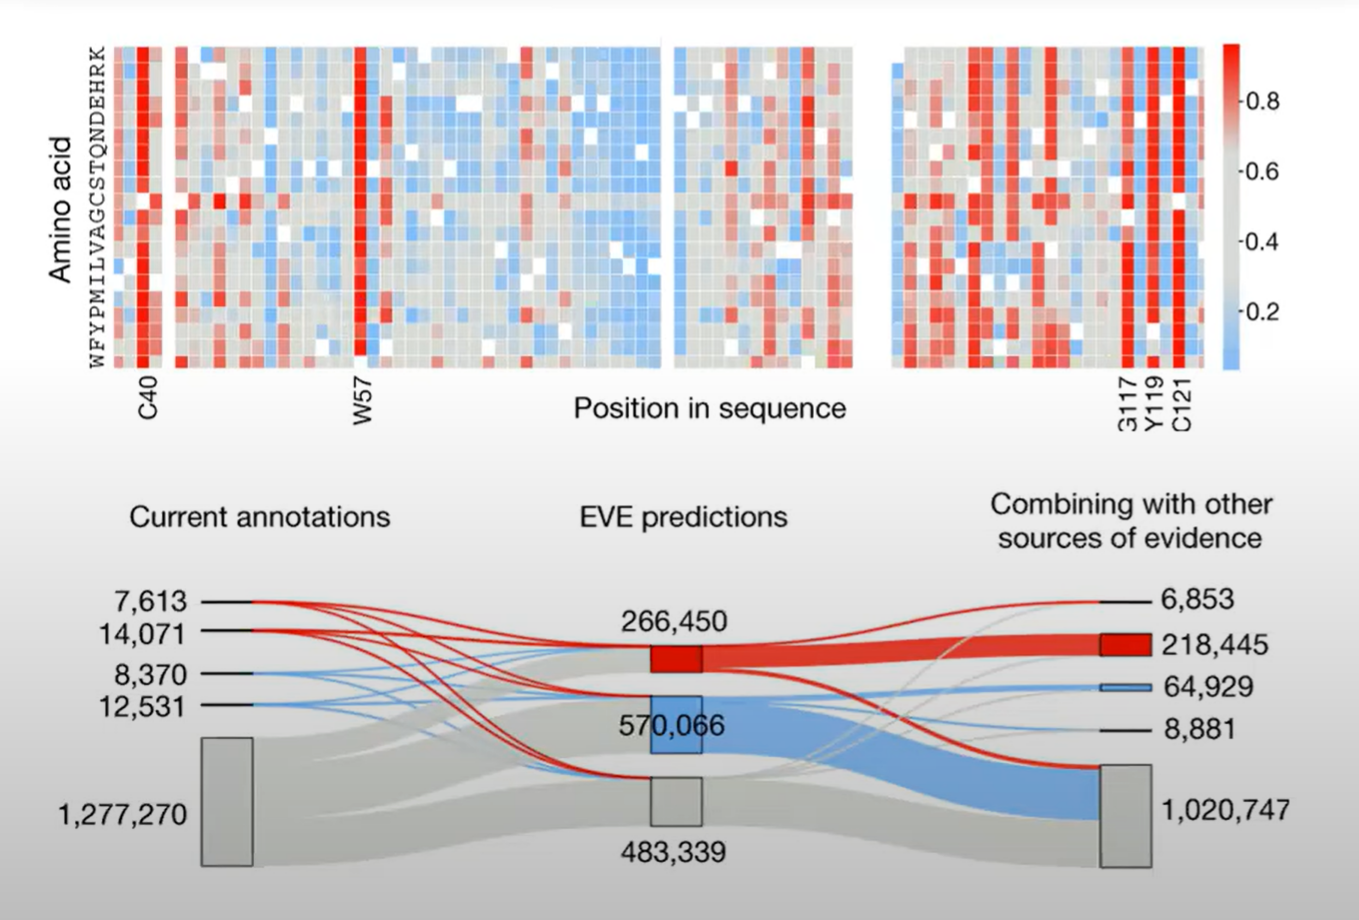
\includegraphics[width=5cm, keepaspectratio]{images/mutation2.png}};
                \node[below=.25cm of mutpic] at (mutpic.south)
                {Predicts whether genetic mutations \\are likely to be disease-causing.};        
            }
             \only<4>{
                % \node {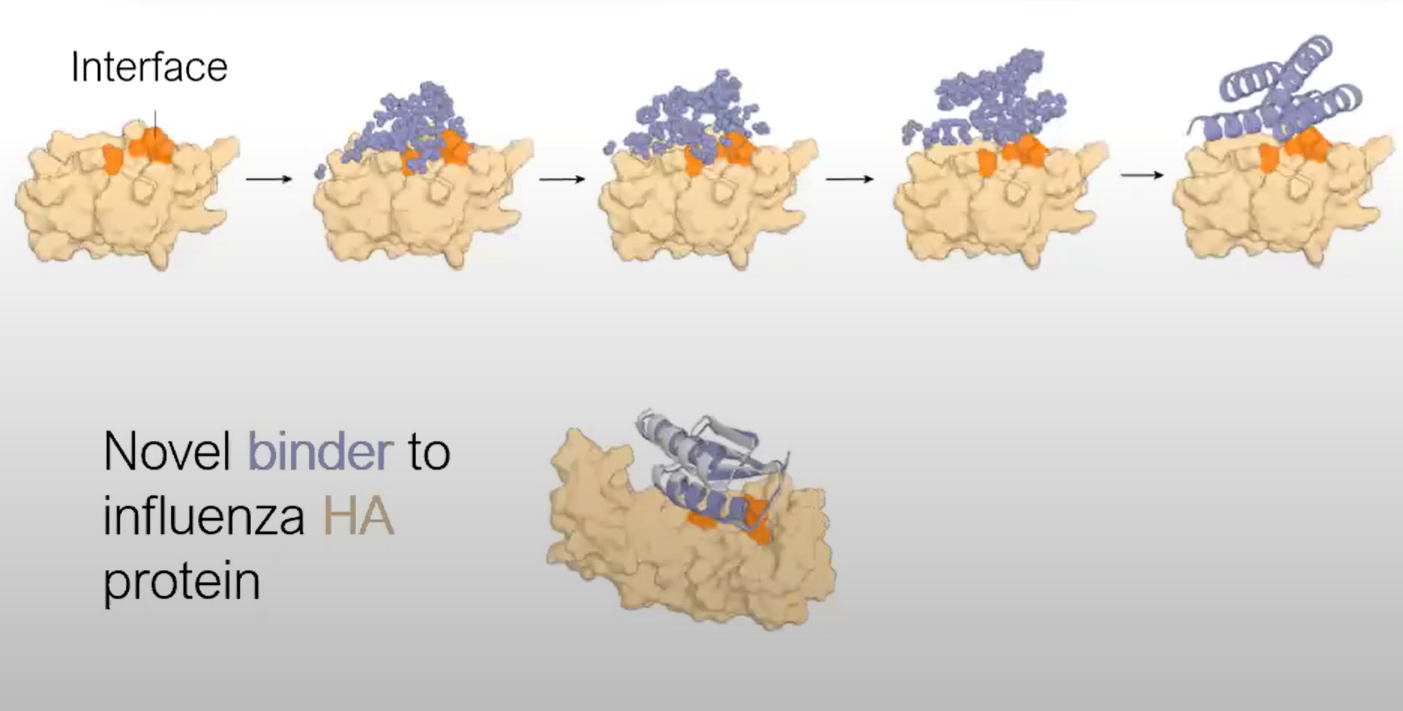
\includegraphics[width=\textwidth]{images/dnovo.png}};
                \node[input,text=black](rose) at (0,3.5)
                {RoseTTAFold};
               \node[below=.25cm of rose] (rosepic) {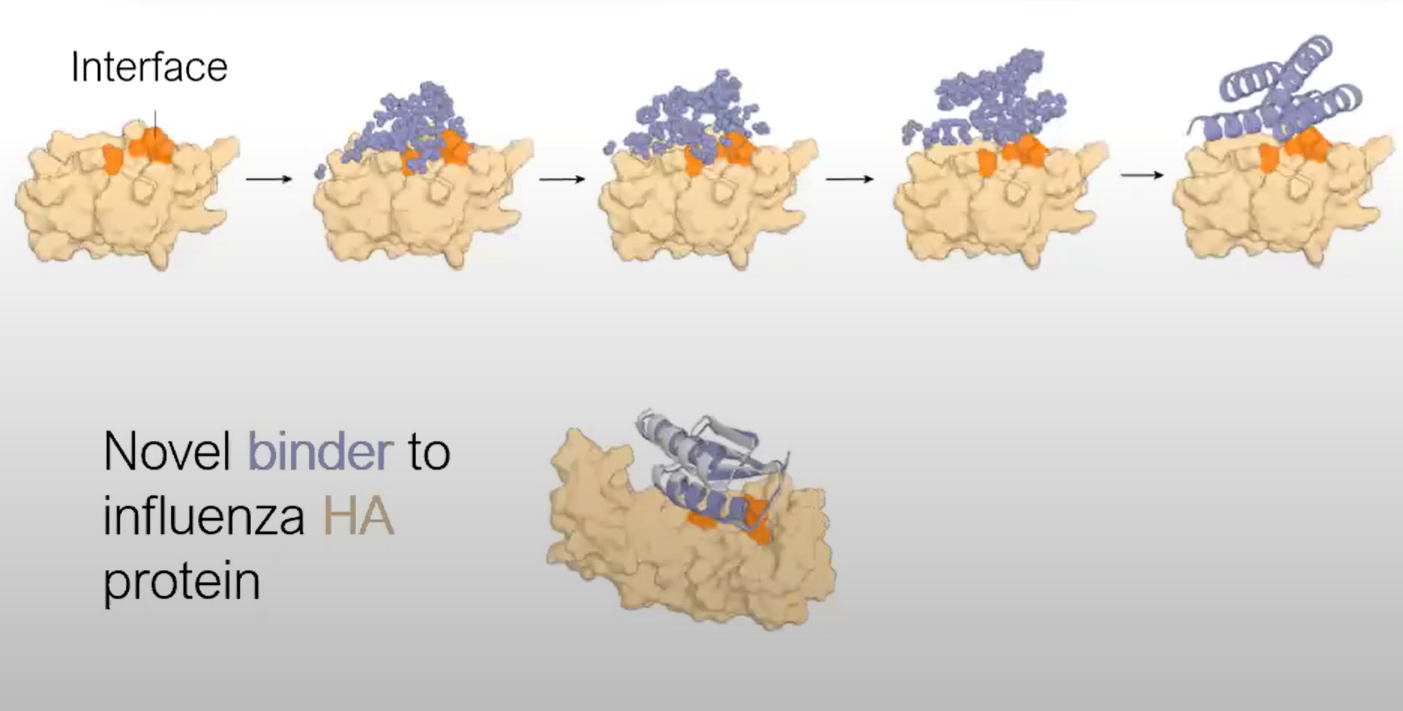
\includegraphics[width=5cm, keepaspectratio]{images/dnovo.png}};
                \node[below=.25cm of rosepic] at (rosepic.south)
                {Enables the design of novel proteins\\ for industrial applications like\\ biofuels, sustainable materials, and \\green chemistry.};  
            }
            

        \end{tikzpicture}
        \end{center}
    \end{columns}
\end{frame}

